\section{Experiments}

\subsection{Search Performance}

\begin{frame}
    \frametitle{Experiment I: Search Performance}

    \begin{itemize}
        \item Compare to random searcher, exhaustive searcher, human searcher with prior knowledge of scenes.
        \item Use held out samples as test set.
        \item Average number of steps on test set.
        \item SPL metric~\cite{anderson_evaluation_2018}, with \(N\) as the number of test samples, \(S_i\) indicating success, \(p_i\) as the number of steps and \(l_i\) as the shortest path length:
    \end{itemize}

    \begin{equation}
        \frac{1}{N} \sum_{i=1}^N S_i \frac{l_i}{\max(p_i,l_i)}
    \end{equation}
\end{frame}

\begin{frame}
    \begin{table}
        \centering
        Gaussian Environment\par\vspace{0.5em}
        \begin{tabular}{lccc}
    \toprule
    Agent & SPL & Success & Length \\
    \midrule
    random & $0.06 \pm 0.01$ & $0.92 \pm 0.06$ & $369.07 \pm 24.93$\\
    greedy & $0.17 \pm 0.00$ & $1.00 \pm 0.00$ & $147.12 \pm 2.38$\\
    exhaustive & $0.21 \pm 0.00$ & $1.00 \pm 0.00$ & $83.37 \pm 2.88$\\
    handcrafted & $0.33 \pm 0.00$ & $1.00 \pm 0.00$ & $65.20 \pm 1.41$\\
    human & $0.23 \pm 0.03$ & $1.00 \pm 0.00$ & $80.97 \pm 13.49$\\
    temporal & $0.24 \pm 0.03$ & $0.99 \pm 0.01$ & $101.25 \pm 13.32$\\
    spatial & $0.29 \pm 0.02$ & $0.99 \pm 0.01$ & $72.16 \pm 5.97$\\
    \bottomrule
\end{tabular}

    \end{table}
\end{frame}

\begin{frame}
    \begin{columns}
        \begin{column}{0.55\textwidth}
            \begin{figure}
                \centering
                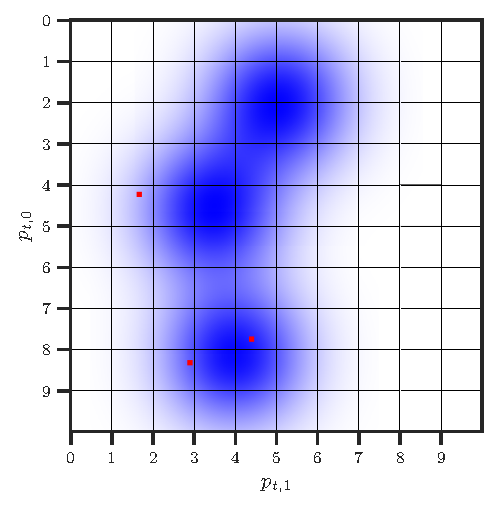
\includegraphics[scale=0.5]{figures/path-scene.pdf}
                \par Environment sample
            \end{figure}
        \end{column}
        \begin{column}{0.5\textwidth}
            \begin{figure}
                \centering
                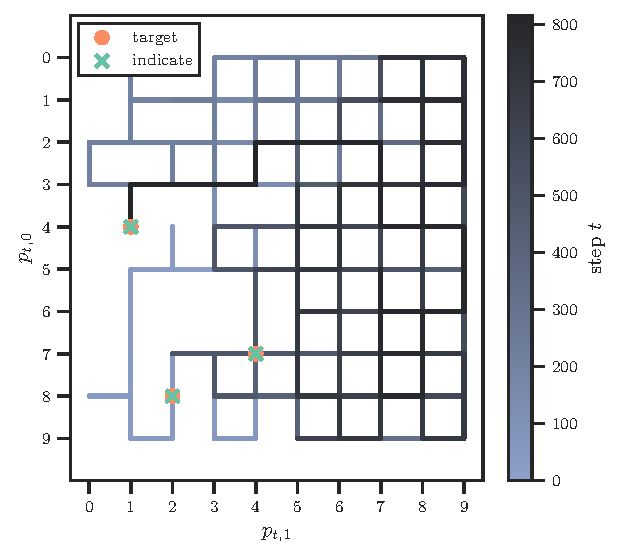
\includegraphics[scale=0.5]{figures/path-random.pdf}
                \par Random baseline
            \end{figure}
        \end{column}
    \end{columns}
\end{frame}

\begin{frame}
    \begin{columns}
        \begin{column}{0.55\textwidth}
            \begin{figure}
                \centering
                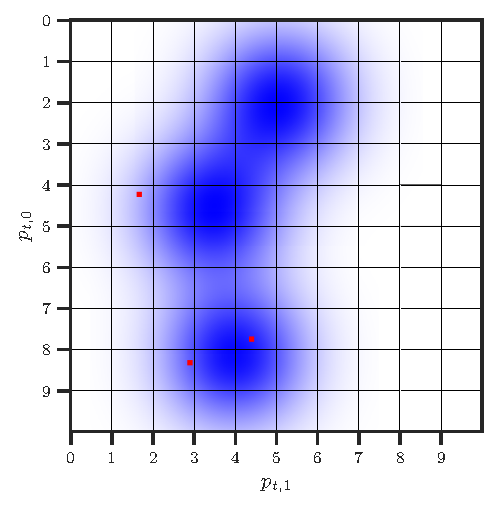
\includegraphics[scale=0.5]{figures/path-scene.pdf}
                \par Environment sample
            \end{figure}
        \end{column}
        \begin{column}{0.5\textwidth}
            \begin{figure}
                \centering
                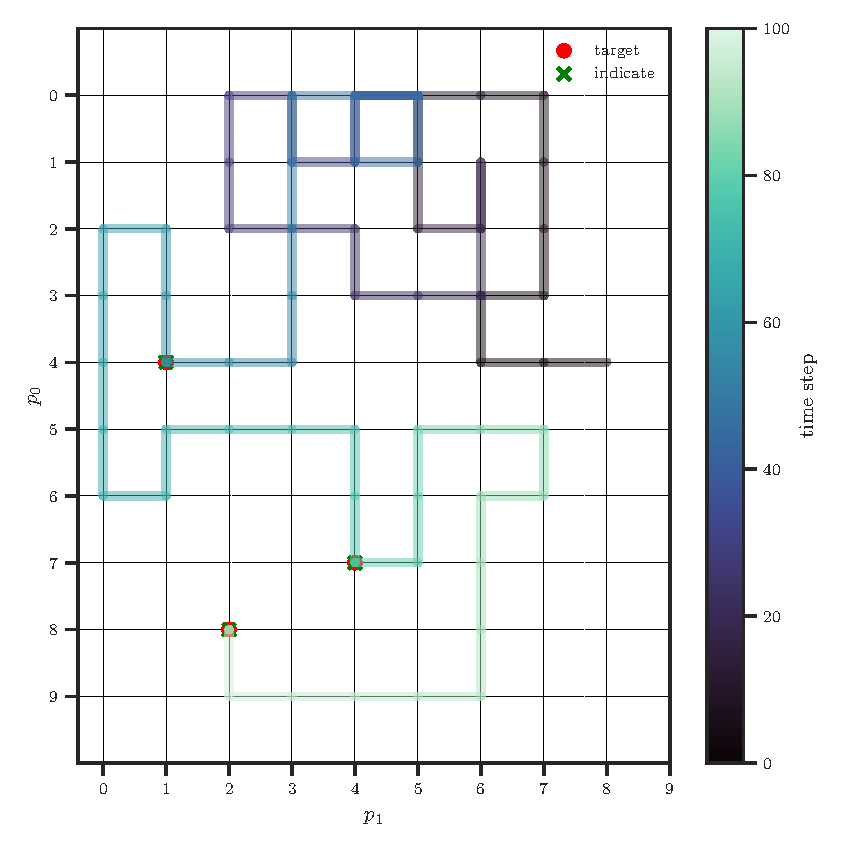
\includegraphics[scale=0.5]{figures/path-greedy.pdf}
                \par Greedy baseline
            \end{figure}
        \end{column}
    \end{columns}
\end{frame}

\begin{frame}
    \begin{columns}
        \begin{column}{0.55\textwidth}
            \begin{figure}
                \centering
                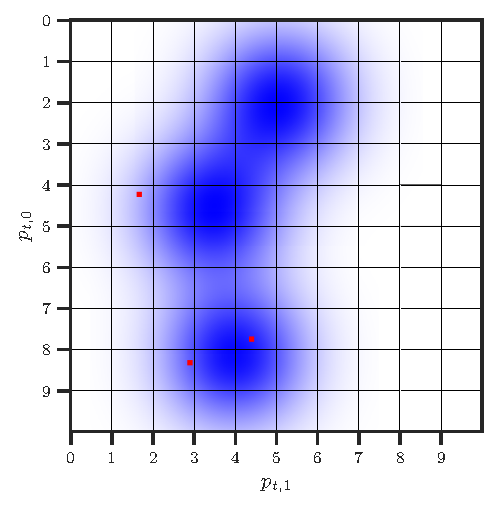
\includegraphics[scale=0.5]{figures/path-scene.pdf}
                \par Environment sample
            \end{figure}
        \end{column}
        \begin{column}{0.5\textwidth}
            \begin{figure}
                \centering
                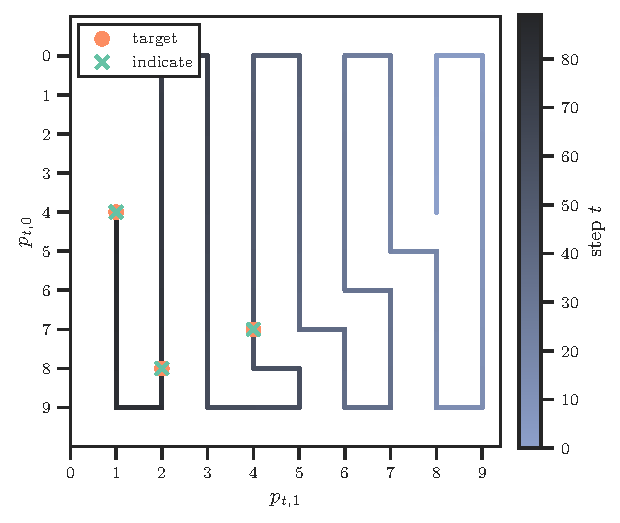
\includegraphics[scale=0.5]{figures/path-exhaustive.pdf}
                \par Exhaustive baseline
            \end{figure}
        \end{column}
    \end{columns}
\end{frame}

\begin{frame}
    \begin{columns}
        \begin{column}{0.55\textwidth}
            \begin{figure}
                \centering
                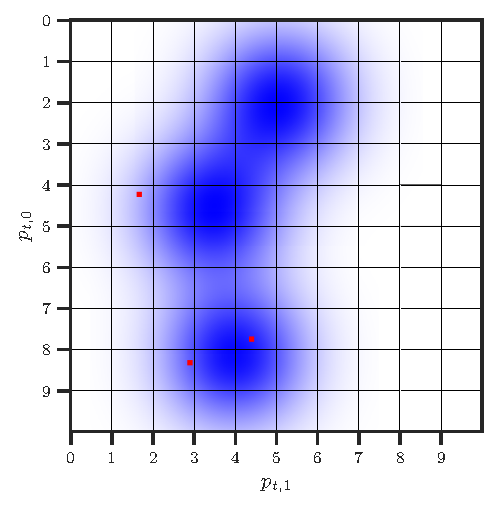
\includegraphics[scale=0.5]{figures/path-scene.pdf}
                \par Environment sample
            \end{figure}
        \end{column}
        \begin{column}{0.5\textwidth}
            \begin{figure}
                \centering
                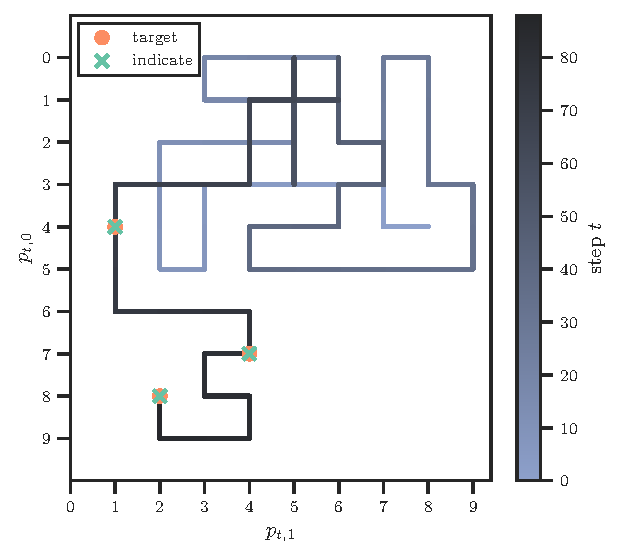
\includegraphics[scale=0.5]{figures/path-handcrafted.pdf}
                \par Handcrafted baseline
            \end{figure}
        \end{column}
    \end{columns}
\end{frame}

\begin{frame}
    \begin{columns}
        \begin{column}{0.55\textwidth}
            \begin{figure}
                \centering
                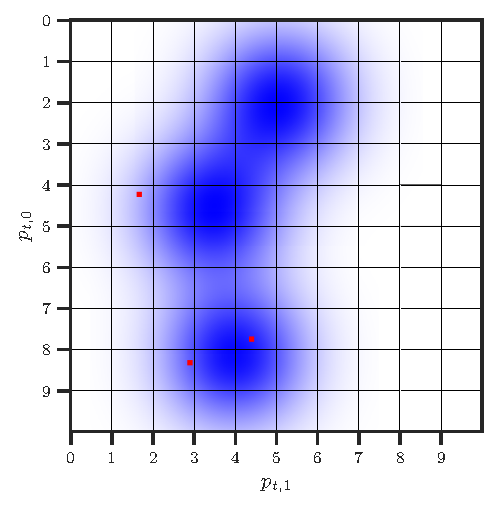
\includegraphics[scale=0.5]{figures/path-scene.pdf}
                \par Environment sample
            \end{figure}
        \end{column}
        \begin{column}{0.5\textwidth}
            \begin{figure}
                \centering
                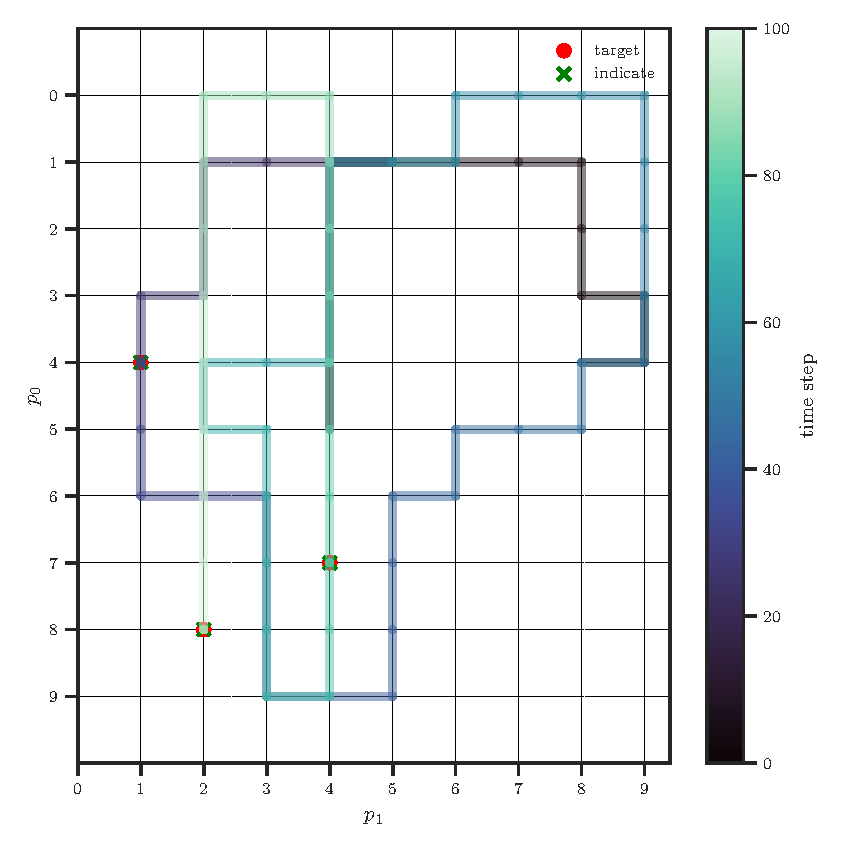
\includegraphics[scale=0.5]{figures/path-lstm.pdf}
                \par Temporal memory
            \end{figure}
        \end{column}
    \end{columns}
\end{frame}

\begin{frame}
    \begin{columns}
        \begin{column}{0.55\textwidth}
            \begin{figure}
                \centering
                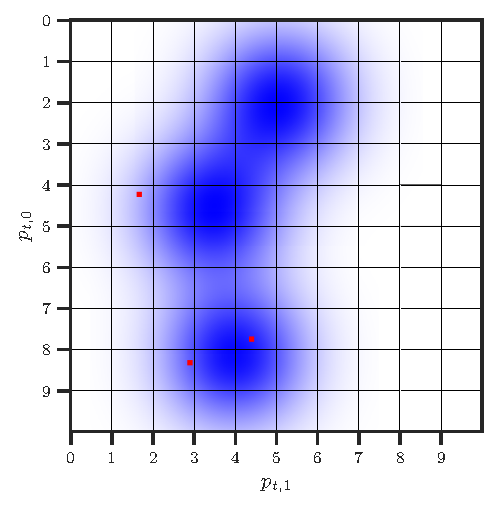
\includegraphics[scale=0.5]{figures/path-scene.pdf}
                \par Environment sample
            \end{figure}
        \end{column}
        \begin{column}{0.5\textwidth}
            \begin{figure}
                \centering
                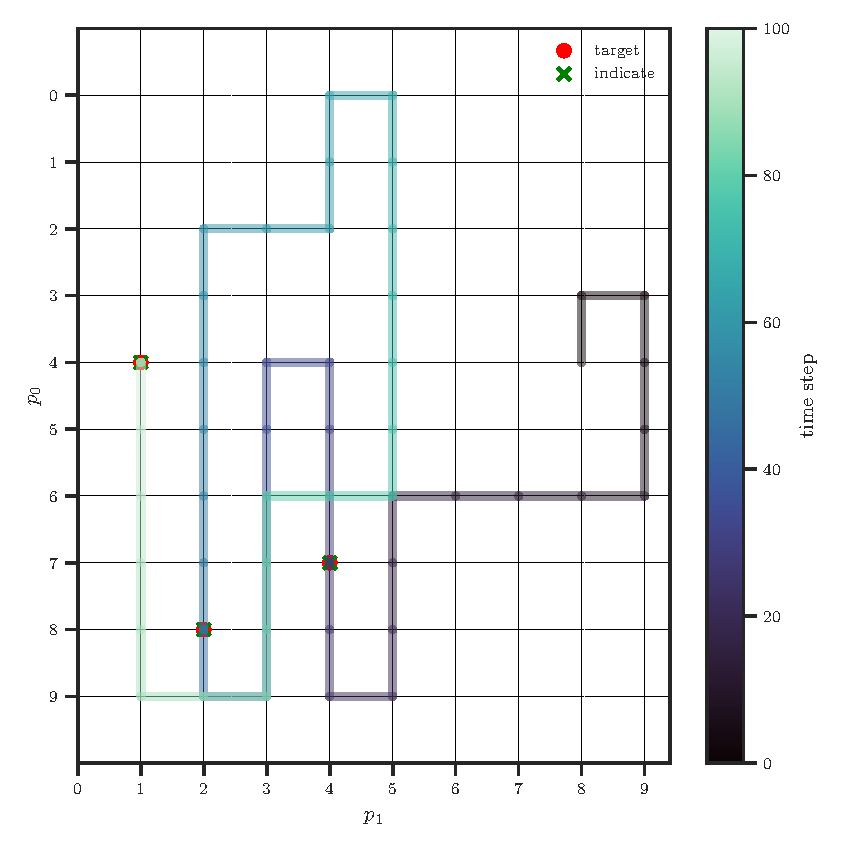
\includegraphics[scale=0.5]{figures/path-map.pdf}
                \par Spatial memory 
            \end{figure}
        \end{column}
    \end{columns}
\end{frame}

\begin{frame}
    \begin{figure}
        \centering
        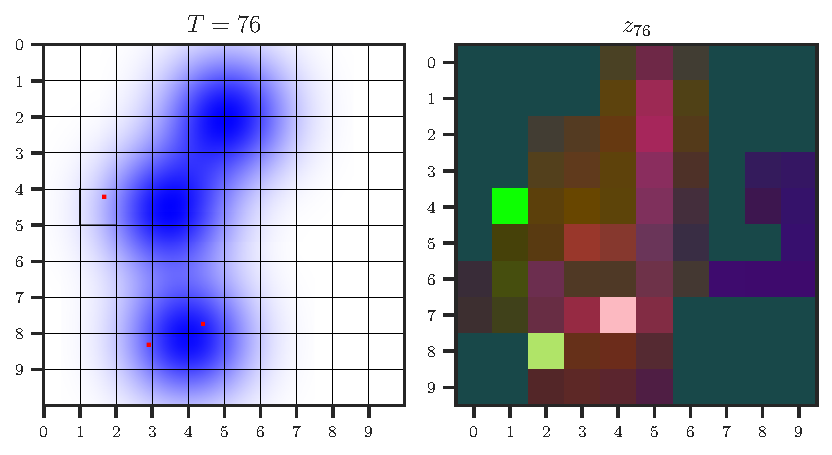
\includegraphics[scale=0.75]{figures/memory-map.pdf}
        \par PCA decomposition of spatial memory after episode.
    \end{figure}
\end{frame}


\begin{frame}
    \begin{table}
        \centering
        Terrain Environment\par\vspace{0.5em}
        \begin{tabular}{lccc}
    \toprule
    Agent & SPL & Success & Length \\
    \midrule
    random & $0.06 \pm 0.01$ & $0.89 \pm 0.04$ & $366.05 \pm 26.96$\\
    greedy & $0.17 \pm 0.01$ & $1.00 \pm 0.00$ & $141.01 \pm 2.31$\\
    exhaustive & $0.22 \pm 0.00$ & $1.00 \pm 0.00$ & $84.11 \pm 0.84$\\
    human & $0.26 \pm 0.02$ & $1.00 \pm 0.00$ & $76.73 \pm 5.33$\\
    \midrule
    temporal & $0.25 \pm 0.02$ & $1.00 \pm 0.01$ & $103.76 \pm 11.69$\\
    spatial & $0.27 \pm 0.01$ & $1.00 \pm 0.00$ & $79.60 \pm 6.88$\\
    \bottomrule
\end{tabular}
    \end{table}
\end{frame}

\begin{frame}
    \begin{table}
        \centering
        Camera Environment\par\vspace{0.5em}
        \begin{tabular}{lccc}
    \toprule
    Agent & SPL & Success & Length \\
    \midrule
    random & $0.04 \pm 0.00$ & $0.62 \pm 0.03$ & $545.09 \pm 56.25$\\
    greedy & $0.12 \pm 0.01$ & $0.97 \pm 0.01$ & $255.60 \pm 10.44$\\
    exhaustive & $0.37 \pm 0.00$ & $1.00 \pm 0.00$ & $67.03 \pm 0.00$\\
    human & $0.68 \pm 0.08$ & $1.00 \pm 0.00$ & $38.10 \pm 5.72$\\
    \midrule
    temporal & $0.70 \pm 0.02$ & $1.00 \pm 0.00$ & $42.36 \pm 2.05$\\
    spatial & $0.66 \pm 0.03$ & $1.00 \pm 0.00$ & $42.90 \pm 1.73$\\
    \bottomrule
\end{tabular}
    \end{table}
\end{frame}

\begin{frame}
    \frametitle{Experiment II: Scaling to Larger Search Spaces}

    \begin{itemize}
        \item Larger search spaces take longer to train:
        \begin{itemize}
            \item More states to explore and exploit.
            \item Stronger demands on memory (remember searched positions, scene understanding).
        \end{itemize}
        \item Investigate impact by comparing agents on \(10 \times 10\), \(15 \times 15\), and \(20 \times 20\) versions of gaussian environment.
    \end{itemize}
\end{frame}

\begin{frame}
    \begin{figure}
        \centering
        \(10 \times 10\)
        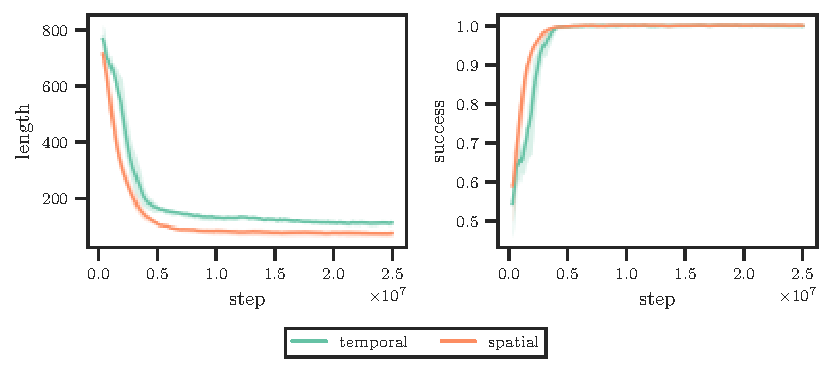
\includegraphics[scale=0.8]{figures/shape-10.pdf}
    \end{figure}
\end{frame}

\begin{frame}
    \begin{figure}
        \centering
        \(15 \times 15\)
        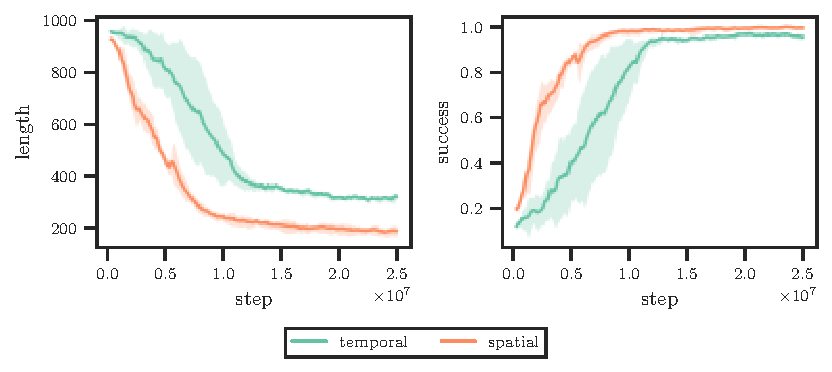
\includegraphics[scale=0.8]{figures/shape-15.pdf}
    \end{figure}
\end{frame}

\begin{frame}
    \begin{figure}
        \centering
        \(20 \times 20\)
        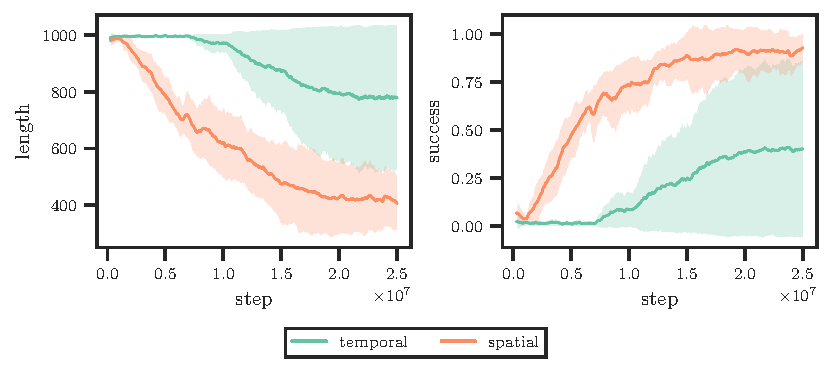
\includegraphics[scale=0.8]{figures/shape-20.pdf}
    \end{figure}
\end{frame}

\begin{frame}
    \frametitle{Experiment III: Generalization From Limited Samples}

    \begin{itemize}
        \item Limit number of scene samples seen during training to 100, 1000, 10 000, \dots.
        \item Use terrain environment, high appearance variance and somewhat realistic.
        \item Fix seed pool used to generate scenes seen during training.
        \item Train agents until convergence (or for a fixed number of time steps).
        \item Test on held out scenes from full distribution. 
    \end{itemize}
\end{frame}

\begin{frame}
    \begin{figure}
        \centering
        10000 samples
        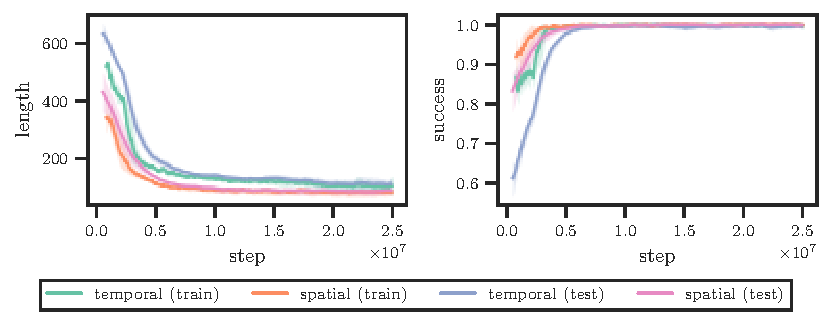
\includegraphics[scale=0.8]{figures/sample-10000.pdf}
    \end{figure}
\end{frame}

\begin{frame}
    \begin{figure}
        \centering
        5000 samples
        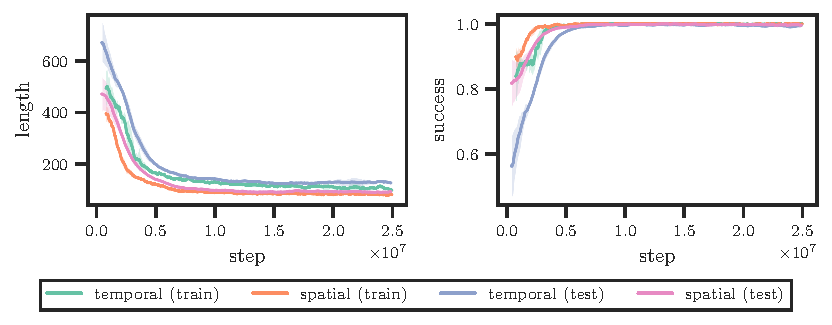
\includegraphics[scale=0.8]{figures/sample-5000.pdf}
    \end{figure}
\end{frame}

\begin{frame}
    \begin{figure}
        \centering
        1000 samples
        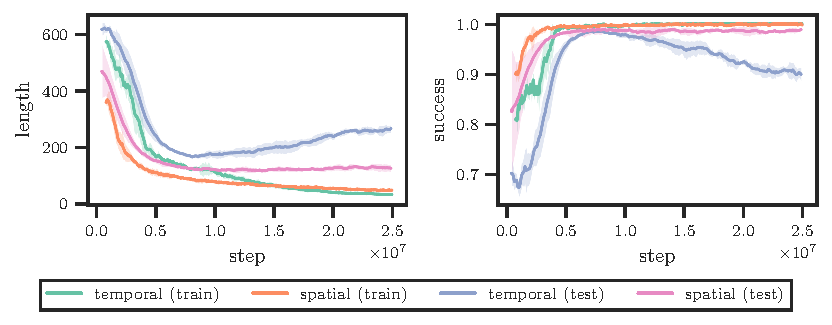
\includegraphics[scale=0.8]{figures/sample-1000.pdf}
    \end{figure}
\end{frame}

\begin{frame}
    \begin{figure}
        \centering
        500 samples
        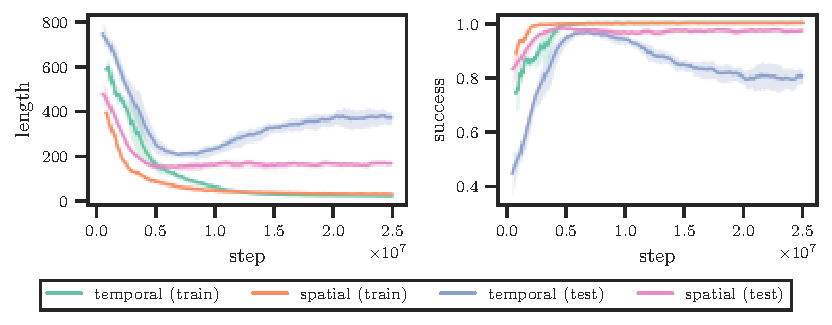
\includegraphics[scale=0.8]{figures/sample-500.pdf}
    \end{figure}
\end{frame}